\documentclass[10pt]{article}

\addtolength{\oddsidemargin}{-.875in}
\addtolength{\evensidemargin}{-.875in}
\addtolength{\textwidth}{1.75in}

\addtolength{\topmargin}{-.875in}
\addtolength{\textheight}{1.75in}

\openup 1em

%macro for commenting
\usepackage{color}
\newcommand{\leo}[1]{{\color{blue}{Leo: #1}}}

% \newcommand{\Xbeta}{ X_i \theta}
\newcommand{\xbeta}{ x_i \beta}
\newcommand{\xtheta}{ x_i \theta}
% \newcommand{\xbetaij}{ x_{ij}^T \theta}
\newcommand{\sgamma}{s_{ij}^T\gamma_i}

\usepackage[round]{natbib}

\usepackage{rotating}
\usepackage{graphicx}
\usepackage{subcaption}

\usepackage{float}
\usepackage{bbm}

\usepackage{amsthm,amsmath, amssymb} 
\usepackage{mathrsfs}
\usepackage{subcaption}
\usepackage{nicefrac}

\usepackage{xcolor}
\newcommand{\aki}[1]{\textcolor{red}{Aki: #1}}

\newtheorem{theorem}{Theorem}
\newtheorem{lemma}{Lemma}
\newtheorem{corollary}{Corollary}
\newtheorem{remark}{Remark}
\newtheorem{example}{Example}


\usepackage{algorithm}
\usepackage{algpseudocode}

%\usepackage{mhequ}
\newcommand{\be}{\begin{equation}\begin{aligned}}
\newcommand{\ee}{\end{aligned}\end{equation}}
\newcommand{\bb}[1]{\mathbb{#1}}
\newcommand{\mc}[1]{\mathcal{#1}}
\DeclareMathOperator{\Binom}{Binomial}
\DeclareMathOperator{\No}{No}
\DeclareMathOperator{\PG}{PG}
\DeclareMathOperator{\IG}{Inverse-Gamma}
\DeclareMathOperator{\Ga}{Gamma}
\DeclareMathOperator{\Bern}{Bernoulli}
\DeclareMathOperator{\U}{Uniform}
\DeclareMathOperator{\Poi}{Poisson}
\DeclareMathOperator{\NB}{NB}
\DeclareMathOperator{\cov}{cov}
\DeclareMathOperator{\var}{var}
\DeclareMathOperator{\diag}{diag}
\DeclareMathOperator{\Diag}{Diag}
\newcommand{\KL}[2]{\textnormal{KL}\left(#1 \parallel #2\right)}
\DeclareMathOperator{\1}{\mathbbm{1}}
\DeclareMathOperator{\bigO}{\mc O}
\newcommand{\dt}{\epsilon} % Stepsize of leapfrog
\newcommand{\mass}{M} % Mass matrix
\newcommand{\hess}{\mathbf{H}} % Hessian notation.



\thispagestyle{empty}
\baselineskip=28pt

\title{\textbf{Extrinsic Priors for Bayesian Modeling with Parameter Constraints}}
\author{Leo Duan, Akihiko Nishimura, David Dunson}
\date{}
\begin{document}
\maketitle
{\bf Abstract:} Prior information often takes for the form of parameter constraints. Bayesian methods include such information through prior distributions having constrained support. By using posterior sampling algorithms, one can quantify uncertainty without relying on asymptotic approximations. However, outside of narrow settings, parameter contraints make it difficult to develop efficient posterior sampling algorithms. We propose a general solution, which relaxes the constraint through the use of an {\em extrinsic prior}, which is concentrated close to the constrained space. General off the shelf posterior sampling algorithms, such as Hamiltonian Monte Carlo (HMC), can then be used directly. We illustrate this approach through multiple examples involving equality and inequality constraints. While existing methods tend to rely on conjugate families, our proposed approach frees us up to define new classes of hierarchical models for constrained problems. We illustrate this through application to a variety of simulated and real datasets.
\vskip 12pt
%\baselineskip=12pt
%\par\vfill\noindent
{\noindent KEY WORDS: Constraint relaxation; Euclidean Embedding; Monotone Dirichlet; Soft Constraint; Stiefel Manifold; Projected Markov chain}
%\par\medskip\noindent
%\clearpage\pagebreak\newpage
\pagenumbering{arabic}


\section{Introduction}
It is extremely common to have prior information available on parameter
contraints in statistical models. For example, one may have prior knowledge
that a vector of parameters lies on the probability simplex or satisfies a
particular set of inequality constraints. Other common examples include
shape constraints on functions, positive semidefiniteness of matrices and
orthogonality. There is a very rich literature on optimization subject to
parameter contraints. One common approach is to rely on Lagrange and
Karush-Kuhn-Tucker multipliers \citep{boyd2004convex}. However, simply
producing a point estimate is often insufficient, as uncertainty
quantification (UQ) is a key component of most statistical analyses. Usual
large sample asymptotic theory, for example showing asymptotic normality of
statistical estimators, tends to break down in constrained inference
problems. Instead, limiting distributions may have a complex form that
needs to be rederived for each new type of constraint, and may be
intractable. An appealing alternative is to rely on Bayesian methods for
UQ, including the constraint through a prior distribution having restricted
support, and then applying Markov chain Monte Carlo (MCMC) to avoid the
need for large sample approximations.

Conceptually MCMC can be applied in a broad class of constrained parameter
problems without complications \citep{gelfand1992bayesian}. However, in
practice, a primary difficulty is designing a Markov transition kernel that
leads to an MCMC algorithm with sufficient computational efficiency to be
practically useful. Common default transition kernels correspond to Gibbs
sampling, random walk Metropolis-Hastings, and (more recently) Hamiltonian
Monte Carlo (HMC). Gibbs sampling relies on alternately sampling from the
full conditional posterior distributions for the different parameters,
ideally in blocks to improve mixing. Gibbs requires the conditional
distributions to be available in a form that is tractable to sample from
directly, limiting consideration to specialized models. In constrained
problems, block updating is typically either not possible or very
inefficient (e.g. relying on rejection sampling with a high rejection
probability), and one-at-a-time updating can lead to extremely slow mixing.
Random walk algorithms provide an alternative, but each step of the random
walk must maintain the parameter constraint. A common approach is to apply
a normal random walk and simply reject proposals that violate the
constraint, but this can have very high rejection rates even if using an
adaptive approach that learns the covariance based on the history of the
chain. An alternative is to rely on HMC. In simple settings in which a
reparameterization can be applied to remove the constraint, HMC can be
applied easily. Otherwise, HMC will generate proposals that violate the
constraint, and hence face problems with high rejection rates in heavily
constrained problems.

Due to the above hurdles, most of the focus in the literature has been on
customized solutions developed for specific constraints.  One popular
strategy is to carefully pick a prior and likelihood such that posterior
sampling is tractable. For example, for modeling of data on manifolds, it
is typical to restrict attention to specific models, such as the
Bingham-von Mises-Fisher distribution for Stiefel manifolds
\citep{khatri1977mises,hoff2009simulation}. For data on the probability
simplex, one instead relies on the Dirichlet distribution. An alternative
is to reparameterize the model to eliminate or simplify the constraint. For
example, when faced with a monotonicity constraint, one may reparameterize
in terms of differences as the resulting positivity constraint leads to
much easier sampling. In the literature on modeling of data on manifolds,
there are two strategies: (i) {\em intrinsic} methods that define a
statistical model directly on the manifold, and (ii) {\em extrinsic}
methods that indirectly induce a model on the manifold through embedding
the manifold in a Euclidean space, defining a model in the Euclidean space,
and then projecting back onto the manifold. Essentially all of the current
strategies for Bayesian modeling with constraints take an intrinsic-style
approach. However, by strictly maintaining the constraint at all stages of
the modeling and computation process, one limits the possibilities in terms
of defining general methods to deal with parameter constraints.

These drawbacks motivate the development of {\em extrinsic} approaches that
define an unconstrained model and/or computational algorithm, and then
somehow adjust for the constraint. A related idea is
\cite{gelfand1992bayesian}, who suggested running Gibbs sampling ignoring
the constraint but only accepting the draws satisfying the constraint.
Unfortunately, such an approach is highly inefficient, as motivated above.
An alternative is to run MCMC ignoring the constraint, and then project
draws from the unconstrained posterior to the appropriately constrained
space. Such an approach was proposed for generalized linear models with
order constraints by \cite{dunson2003bayesian}, extended to functional data
with monotone or unimodal constraints \citep{gunn2005transformation}, and
recently modified to nonparametric regression with monotonicity
\citep{lin2014monogp} or manifold \citep{lin2016extrinsic} constraints.

An alternative idea is to {\em relax} a sharp parameter constraint by
defining a prior that has unrestricted support but places small probability
outside of the constrained region. \cite{neal2011mcmc} suggested such an
approach to apply HMC in settings involving a simple truncation constraint,
while \cite{pakman2014exact} applied a related idea to improve sampling
from truncated multivariate normal distributions.

The goal of this article is to dramatically generalize these specific
approaches to develop a broad class of {\em extrinsic priors} for parameter
constrained problems. These priors are defined to place small probability
outside of the constrained region, while permitting use of efficient and
general use MCMC algorithms; in particular, HMC. Unlike intrinsic methods,
such as Riemannian and geodesic HMC
\citep{girolami2011riemann,byrne2013geodesic}, our approach is simple to
implement in general settings using automatic algorithms. The generality
frees up a much broader spectrum of Bayesian models, as one no longer needs
to focus on very specific computationally tractable models.  Theoretic
studies are conducted and original models are shown in simulations and data
applications.

\section{Conditional Constrained Bayes Methodology}

\subsection{Deriving Constrained Distribution via Conditioning}

Let $\theta \in \mc D$ denote the parameters of interests. The support $\mc
D$ is a constrained space. The usual Bayesian approach assigns a prior
density $\pi_{0,\mc D}(\theta)$ for $\theta$ only having support $\mc D$. A
simple strategy is to reparameterize the constrained space in terms of
parameters $\theta^*$ in a less constrained space (such as Euclidean
space), with the constraint induced. The reparameterization
$\theta\rightarrow\theta^*$ is often known as `embedding' in manifold
literature \citep{nash1954c1,nash1956imbedding}.  Although this strategy
often works, reparameterization makes it difficult to maintain certain
property in $\mc D$, such as uniformity on a manifold as described by
\cite{diaconis2013manifold}; also, such a convenient reparameterization is
not always available, especially when $\mc D$ is the intersection of two or
more different types of constrained space.

On the other hand, in un/less-constrained space, there is a large family of
distributions  with well-studied properties. We present a new strategy to
adapt them into the constrained space. Starting with a distribution of
density $\pi_{\mc R}(\theta)$ on a encompassing space $\mc R\supset \mc D$,
we focus on constrained space that can be defined as $\mc D =\{\theta:
v(\theta)={\bf 0}\}$ with $v: \bb{R}^p\rightarrow \bb  R^d$ Lipschitz and
measurable with respect to $\pi_{\mc R}(\theta)$. Although this imposes a
restriction, there is a rich class within this category. For each
measurable function $f:\mc R\rightarrow \bb R$, one can use
$v(\theta)=f(\theta)$ for equality constraint $f(\theta)=0$, and
$v(\theta)=|f(\theta)|_+=\left\{\begin{array}{cc}  0 \text{ if } f(x)\le 0
\\ f(x) \text{ if } f(x)> 0\end{array}\right.$ for inequality constraint
$f(\theta)<0$.

The constrained density can then be derived as the conditional density given the
value of $v(\theta)$ equal to $\bf 0$

\be
\pi_{\mc D}(\theta)=\pi_{\mc R}(\theta\mid v(\theta)={\bf 0})\propto \pi_{\mc R}(\theta) \mathbbm{1}_{\theta\in \mc
D}/J(v(\theta))
\ee
where $\mathbbm{1}(\theta\in\mc D)$ is an indicator function equal $1$ when
$\theta\in \mc D$ and $0$ otherwise; $J(v(\theta))$ is induced by the
transformation, which equals to
$\sqrt{\mbox{det}D(v(\theta))'
D(v(\theta))}$ with $D(v(\theta))$ the partial derivative matrix. This is based on the area
formula in \citep{federer2014geometric} and a more rigorous justification
is deferred to the theory section.

We now provide some concrete illustration of this approach. Consider prescribing
a distribution on a unit hypersphere $\{\theta:
\theta'\theta=1\}$ inside $\bb R^p$. We start with a familiar
location-scale distribution Gaussian distribution with diagonal
covariance $\theta \in \No(F,I\sigma^2)$ as $\pi_{\mc
R}$ ($F\in \bb R^p$). Conditioning on $v(\theta)=\theta'\theta-1=0$ yields

\be
\pi_{\mc D}(\theta) &\propto
\exp(-\frac{\theta'\theta}{2\sigma^2}+\frac{F'\theta}{\sigma^2})
\mathbbm{1}_{\theta'\theta=1}/2 \\
& \propto
\exp(\frac{F'}{\sigma^2}\theta)
\mathbbm{1}_{\theta'\theta=1}
\ee
where the quadratic term of $\theta$ is left out as a constant under
the constraint; $J(v(\theta))=2$. This gives rise to the famous von
Mises--Fisher distribution \citep{khatri1977mises}. As the center and
concentration is determined by the location $F$ and scale-inverse
$\sigma^{-2}$ in Gaussian $\pi_{\mc
R}(\theta)$, this pattern is inherited in the conditional
(Figure~\ref{sphere_examples}(a)); in directional statistics, the
normalized ${F}/{\|F\|}$ is called the mean
direction (when $\|F\|\neq \bf 0$) and $\|F\|/\sigma^2$ is called
concentration parameter \citep{khatri1977mises}.

This immediately suggests one can choose different $\pi_{\mc R}(\theta)$
based on its properties in unconstrained space $\mc R$, and induce similar behavior on the $\mc D$. Starting from
correlated Gaussian $\theta \in \No(F,\Sigma)$, one obtains 
\be
\pi_{\mc
D}(\theta) & \propto\exp(-\frac{1}{2}\theta'\Sigma^{-1}\theta+
{F'}{\Sigma^{-1}}\theta) \mathbbm{1}_{\theta'\theta=1} \\
& \propto \exp(\sum_{k=2}^p(-\frac{1}{2}w_k)\theta'\Psi_k'\Psi_k\theta
+ (-\frac{1}{2}w_1)\theta' \Psi_1\Psi'_1\theta+
+ \sum_{k=1}^p w_k F'\Psi_k\Psi'_k\theta ) \mathbbm{1}_{\theta'\theta=1} \\
& \propto \exp(-\frac{1}{2}\sum_{k=2}^p( w_k - w_1)\theta'\Psi_k'\Psi_k\theta
+ \sum_{k=1}^p w_k F'\Psi_k\Psi'_k\theta )\mathbbm{1}_{\theta'\theta=1}
\ee
where $\Psi_k$ and $w_k$ are the $k$th eigenvector and eigenvalue of $\Sigma^{-1}$. This is the $p$-dimensional generalization of the Fisher-Bingham distribution
\citep{mardia1975statistics}, which has $p=3$. Similar to their roles in Gaussian covariance,
the eigenvectors control axes of the ellipse on the sphere
\citep{kent1982fisher}. An illustration with correlated $x$ and $y$ axes is shown in
Figure~\ref{sphere_examples}(b).

Alternatively, one can start from a
multivariate $t$-distribution $t_m(F,I\sigma^2)$ with $m$ degrees of freedom,
mean $F$ and variance $I\sigma^2$, and obtain constrained density 
\be
\pi_{\mc
D}(\theta)\propto
(1+\frac{1+F'F}{m\sigma^2}-\frac{2F'\theta}{m\sigma^2})^{-{(m+p)}/{2}}\mathbbm{1}_{\theta'\theta=1}
\ee
Similar to the relation between $t$-distribution and Gaussian, at small
$m$, the induced distribution (Figure~\ref{sphere_examples}(c) with $m=3$) exhibits less concentration than von
Mises--Fisher on the sphere.

\begin{figure}[H]
\begin{subfigure}[b]{0.30\textwidth}
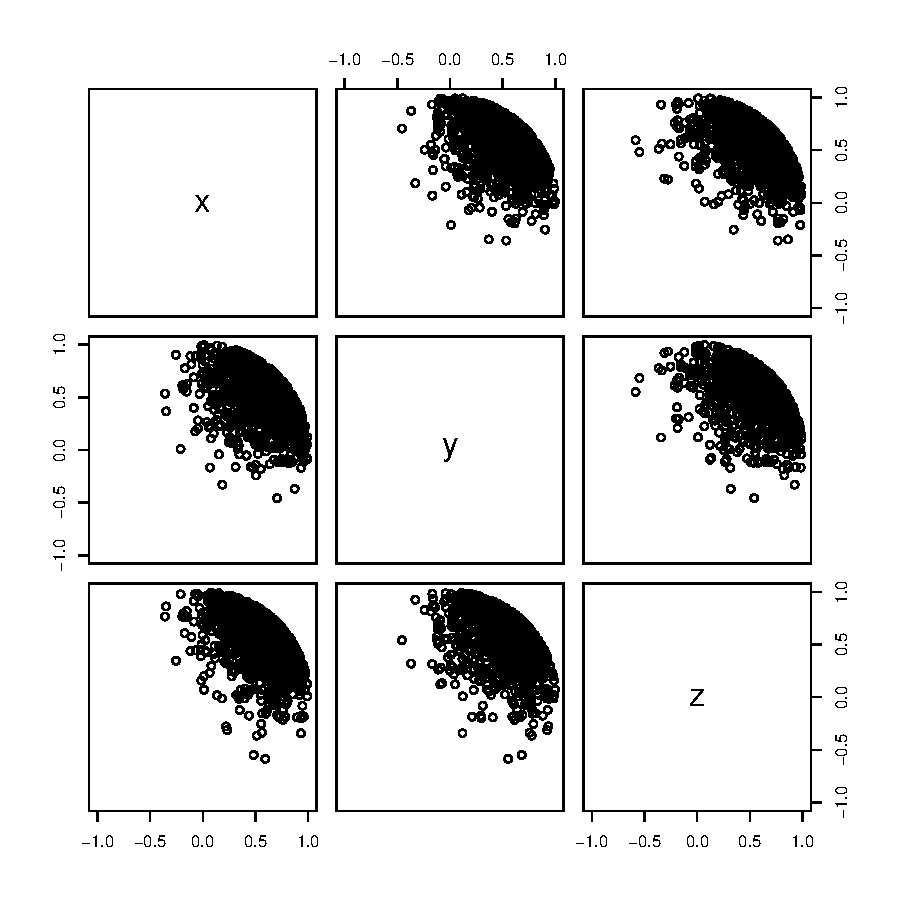
\includegraphics[width=1\textwidth]{sphere_vmf}
\caption{Constrained independent Gaussian distribution}
\end{subfigure}
\begin{subfigure}[b]{0.30\textwidth}
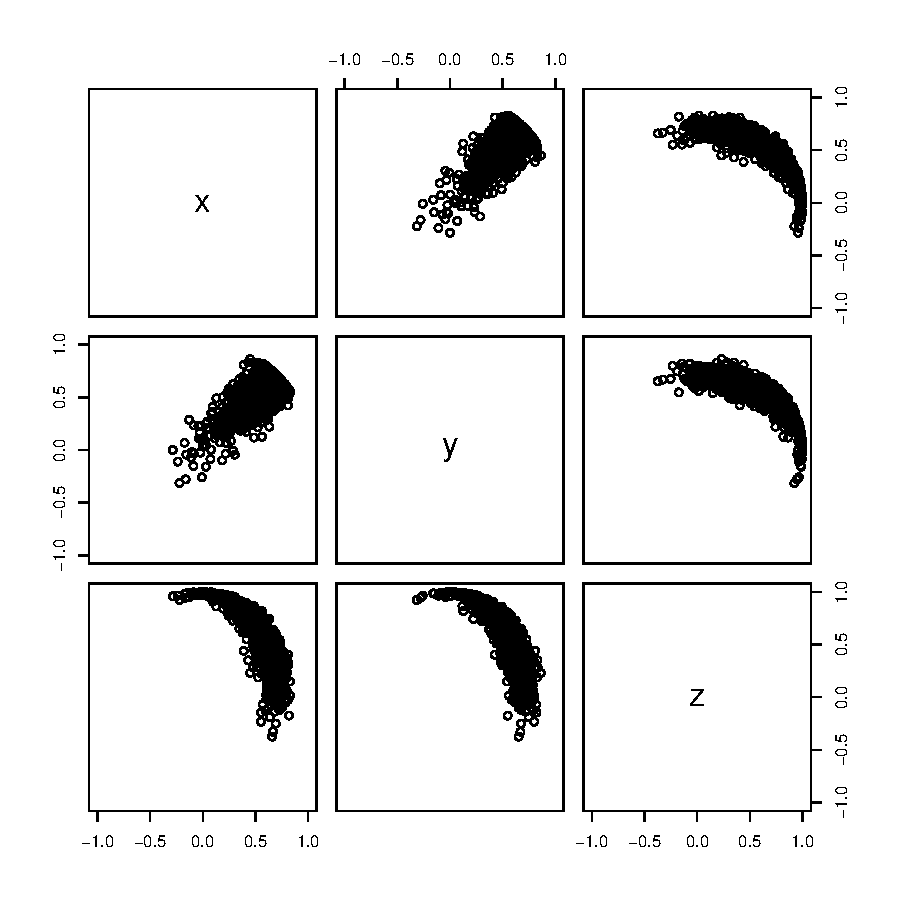
\includegraphics[width=1\textwidth]{sphere_fb}
\caption{Constrained correlated Gaussian distribution}
\end{subfigure}
\begin{subfigure}[b]{0.30\textwidth}
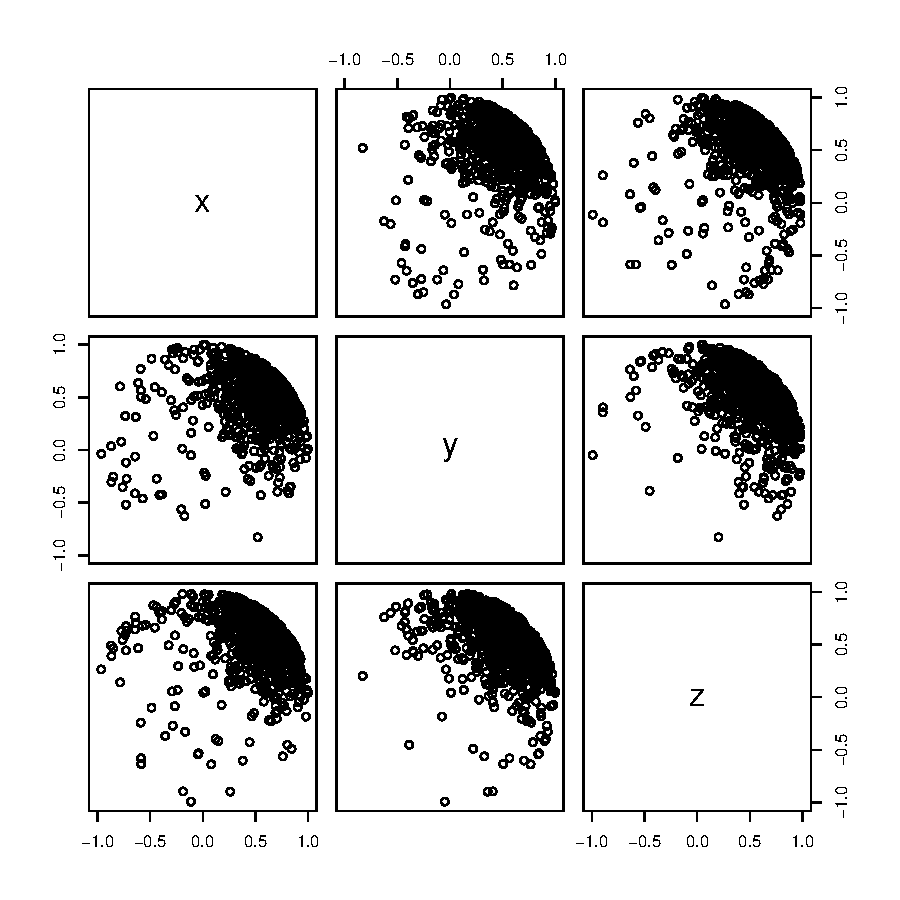
\includegraphics[width=1\textwidth]{sphere_t}
\caption{Constrained independent $t_3$ distribution}
\end{subfigure}
\caption{Sectional view of random samples from constrained distributions on a unit sphere inside $\bb R^3$. The distributions are derived through conditioning on $\theta'\theta=1$ based on unconstrained densities of (a) $\No( F, \diag\{0.1\})$, (b) $\No(F, \left[\protect\begin{smallmatrix} 0.1 & 0.09 & 0 \\ 0.09 & 0.1 & 0 \\ 0 & 0 &0.1  \protect\end{smallmatrix}\right])$, (c) $t_3(F,\diag\{0.1\} )$, where $F=[1/\sqrt{3},1/\sqrt{3},1/\sqrt{3}]'$.}
\label{sphere_examples}
\end{figure}

\subsection{Constraint Relaxation for Posterior Inference}

When the constrained distribution in last section is used as a prior,
one can obtain posterior:
\be
\label{exactPosterior}
\pi(\theta\mid y) & \propto L(y;\theta)\pi_{\mc D}(\theta) \\
& \propto L(y;\theta) \pi_{\mc
R}(\theta) /J(v(\theta))\mathbbm{1}_{\theta\in \mc D},
\ee
where $L(y;\theta)$ denotes the likelihood with $y$ the data. As the
normalizing term in prior is canceled, the posterior takes a simple form
with the unconstrained density and $J(v(\theta))$. On the other hand, the
posterior also has support only inside $\mc D$ due to the inheritance of
$\mathbbm{1}_{\theta\in \mc D}$ from $\pi_{\mc D}(\theta)$. Unfortunately,
the indicator often poses a challenge for posterior inference. 

We now present an approximation to the sharp indicator, relaxing support into a
neighborhood surrounding $\mc D$,

\be
\label{approximatePosterior}
\tilde{\pi}(\theta\mid y)  & = \frac{1}{m(\lambda)} L(y;\theta) \pi_{\mc
R}(\theta) /J(v(\theta)) \exp (- \sum_{k=1}^K |v_k(\theta)|^\alpha/\lambda_k),
\ee
where $v_k$ is the $k$th equation in $v(\theta)$, $\lambda_k\ge 0$ is a
tuning parameter that controls the amount of relaxation, $\alpha$ is
typically chosen as $1$ or $2$, $m(\lambda)$ is an unknown normalizing
constant such that $\int_{\mc R} \tilde{\pi}(\theta\mid y) d\theta=1$.
When $\theta\in \mc D$, \eqref{approximatePosterior} is proportional to
\eqref{exactPosterior}; when $\theta\not\in \mc D$,
\eqref{approximatePosterior} has positve density, providing constraint
relaxation. When $\lambda_k=0$ for all $k$, \eqref{exactPosterior} and
\eqref{approximatePosterior} are equal.

To illustrate this relaxation, consider a posterior from a sum-constrained
bivariate Gaussian random vector $[\theta_1,\theta_2]' \mid y \sim \No(0,I)
\mathbbm{1}_{\theta_1+\theta_2-1=0}$. Using
$v(\theta)=\theta_1+\theta_2-1=0$ for the
constraint, $J(v(\theta))=\sqrt 2$, \eqref{exactPosterior} is proportional to 
$$
\phi(\theta_1)
\phi(\theta_2)\mathbbm{1}_{v(\theta)=0}
$$
where $\phi(.)$ is the standard
normal density. In this simple example, the exact posterior density has closed-form
as

$$
\pi(\theta\mid y)=\frac{\sqrt{2}}{\sqrt{2\pi}} \exp(-\frac{(\theta_1-\frac{1}{2})^2}{2/2})
\mathbbm{1}_{\theta_2=1-\theta_1}
$$
corresponding to $\theta_1\mid (\theta_1+ \theta_2=1) \sim
\No(1/2,1/2)$, $\theta_2\mid \theta_1 \sim \delta_{1-\theta_1}(.)$.
Equivalently, it follows a degenerate bivariate Gaussian distribution:
$$\begin{bmatrix} \theta_1 \\ \theta_2 \end{bmatrix} \sim
\No_{\text d} \left(
\begin{bmatrix} \frac{1}{2} \\ \frac{1}{2} \end{bmatrix},
\begin{bmatrix} \frac{1}{2} & -\frac{1}{2}  \\  -\frac{1}{2}  & \frac{1}{2} \end{bmatrix}
\right).$$

Using constraint relaxation $ \exp( - (\theta_1+\theta_2-1)^2/\lambda)$ to
replace $\mathbbm{1}_{v(\theta)=0}$, we obtain approximation $\theta_1 \sim \No(\frac{2}{\lambda+4},\frac{\lambda+2}{\lambda+4})$, $\theta_2\mid \theta_1 \sim \No(\frac{2}{\lambda+2}(1-\theta_1),\frac{\lambda}{\lambda+2})$. Marginally, 

$$\begin{bmatrix} \theta_1 \\ \theta_2 \end{bmatrix} \sim
\No \left(
\begin{bmatrix} \frac{2}{\lambda+4} \\ \frac{2}{\lambda+4} \end{bmatrix},
\begin{bmatrix} \frac{\lambda+2}{\lambda+4} & -\frac{2}{\lambda+4}  \\  -\frac{2}{\lambda+4}  &\frac{\lambda+2}{\lambda+4} \end{bmatrix}
\right).$$
Clearly the approximation density becomes exact when $\lambda\rightarrow 0$.

\subsection{Reparameterization based on Constrain Relaxation}
It is possible for some cases to use constraint relaxation for reparameterization of $\eqref{exactPosterior}$ instead of approximation. Although the application is more limited, it still covers a large range of useful constraints, such as simplex. The idea is to consider the constrained $\theta$ as the projection of unconstrained parameter $\theta^*$. Coupled with an extra parameter $w$, one could form a bijective mapping between $\{\theta,w\}$ and $\{\theta^*, w\}$, and obtain variable transformation in the density. For example, $\theta$ can be a simple rescaling $\theta^*/\|\theta^*\|_1$ and $w=\|\theta^*\|_1$. Using the mapping, one can reparameterize the exact posterior \eqref{exactPosterior} using less constrained $\theta^*$.

To provide concrete explanation, we illustrate the rescaling case via a $(p-1)$-simplex example
$\{\theta:  \sum_{i=1}^p\theta_k=1, \theta_i\in(0,1) \text{ for } i=1,\ldots,p\}$, using Dirichlet distribution 
\be
\pi_{\mc D}(\theta)\propto \prod_{i=1}^p \left(\theta_i^{\alpha-1}\mathbbm{1}_{\theta_i\in(0,1)} \right)\mathbbm{1}_{\sum_{i=1}^p\theta_k=1}.
\ee
Relaxing the $1$-norm constraint into space $\mc R=[0,1]^p$, one would have $\sum_{i=1}^p\theta^*_k=w$. A bijective mapping exists $\{ \theta_1= \theta_1^*/w,\theta_2= \theta_2^*/w,\ldots, \theta_{p-1}= {\theta_{p-1}^*}/{w}, w= w\}$ and substitute into the original density, one would obtain 
\be
(1-\frac{\sum_{i=1}^{p-1} \theta^*_i}{w})	\prod_{i=1}^{p-1} (\frac{\theta_i^*}{w})^{\alpha-1}  w^{-(p-1)}
\ee
where $w^{-(p-1)}$ is the Jacobian of transforming from $\{\theta_1,\ldots,\theta_{p-1},w\}$ to $\{\theta^*_1,\ldots,\theta^*_{p-1},w\}$.


avoid incurring approximation error at all by reparameterize the original constrained
parameters as the projection of the parameters under constraint
relaxation. This 

For example, in the previous sum-constraint Gaussian example, one could


original $\theta$ in terms of the 


\subsection{Properties}

We now present the properties of the proposed approach. We first establish
that the conditioning approach yields valid probability measure.

We focus on $\mc R$ being a $p$-dimensional Euclidean space and the
intrinsic dimension of $\mc D$, $\mbox{dim}(\mc D)=d\le p$ and is integer.
When $d<p$, the
$p$-dimensional Lebesgue measure $\mu^p(\mc D)=0$. To maintain the definition
of conditional probability, we utilize the concept of {\it regular
conditional probability} (r.c.p.)
\citep{kolmogorov1950foundations}. For this article to be self-contained,
we list the definition \citep{leao2004regular} as below.

Let $(X, \mathscr A, \mu)$ be a probability space and $(Y, \mathscr B)$ a measurable space. With a measurable function $v:X\rightarrow Y$, $v^{-1}(\mathscr B)\in \mathscr A$.
A r.c.p is a function
$f: Y\times \mathscr A \rightarrow[0,1]$ satisfying:

\begin{enumerate}
	\item $f(y, .)$ is a measure on $(X,\mathscr A)$ for each $y \in
	Y$;
	\item $f(., E)$ is a measurable function on $(Y,\mathscr B)$ for each $E\in \mathscr A$;
	\item For each $E \in \mathscr A$, $F\in \mathscr B$,
	$\mu(E \cap v^{-1}(F))=\int_{F} f(y, E) \mu_y(dy)$, with
	$\mu_y$ the induced measure on $(Y,\mathscr B)$.
\end{enumerate}

Using the previous notation, we write $f(y,E)= P(\theta\in E\mid
v(\theta)=y)=\int_E \pi_{\mc R}(\theta
\mid v(\theta)=y) d\theta$

\begin{remark}
Assuming $J(v(\theta))\neq 0$ and there is a finite and
non-negtive integer $s$ such
that, for some $y\in Y$,
\be
m_s(y)=\int_{\bb R^s} \frac{\pi_{\mc
R}(\theta)
\mathbbm{1}_{v({\theta})=y}}{J(v(\theta))}d\theta\in(0,\infty),
\ee
then
\begin{equation}
P(E\mid v(\theta)=y)=\left\{\begin{array}{ll}  \frac{1}{m_s(y)}\int_{E \cap \bb R^s} \frac{\pi_{\mc
R}(\theta) \mathbbm{1}_{v({\theta})=y}}{J(v(\theta))}d\theta
& \text{  , if }m_s(y)\in(0,\infty) \\
\delta_{x^*}(E) \text{ with fixed } x^*\in \bb R^p
& \text{  , if }m_s(y)\in\{0,\infty\} \\
\end{array}\right.
\end{equation}
is a valid r.c.p..
\end{remark}
\begin{proof} The first two crieria for r.c.p are trivally satisfied. Hausdorff measure is the standard tool for geometric measure theory \citep{federer2014geometric}, defined as $\mc H^{s}(A)= \underset{\delta\rightarrow 0}\lim \inf \{ \sum \left[{\text{diam}(S_i)}\right]^s: {A\subseteq \cup S_i, \text{diam}(S_i)\le \delta}, \text{diam}(S_i)=\sup_{x,y\in S}\|x-y\|\}$. We denote the normalized Hausdorff measure as $\bar{\mc H}^{s}(A) =\frac{\Gamma(\frac{1}{2})^{s}}{2^s \Gamma(\frac{s}{2}+1)} \mc H^{s}(A)$. When $s$ is an integer, Lebesgue and normalized Hausdorff measures coincide  $\mu(A)= \bar{\mc H}^{s}(A)$ \citep{evans2015measure}.

Similar to the proof of (2) of Proposition 2 of \cite{diaconis2013manifold}, using co-area formula \citep{federer2014geometric}:

\be
\mu(E\cap v^{-1}(F))= & \int_{\bb R^p} \mathbbm{1}_{\theta \in E} \mathbbm{1}_{\theta \in v^{-1}(F)}\pi_{\mc R}(\theta) d\theta \\
= & \int_{\bb R^{p-s}} \left[ \int_{v^{-1}(y)} \mathbbm{1}_{\theta \in E} \mathbbm{1}_{v(\theta) \in F}  \frac{ \pi_{\mc R}(\theta)}{J(v(\theta))} \bar{\mc H}^{s}(d\theta)\right] dy \\
= & \int_{F\cap \bb R^{p-s}} \left [ \int_{ E \cap \bb R^{s}}  \frac{ \pi_{\mc R}(\theta) \mathbbm{1}_{v(\theta)=y}}{J(v(\theta))} d\theta  \right] dy \\
\ee


For $y\in \{y':m(y')=0\}$, $\int_{ E \cap \bb R^{s}}  \frac{ \pi_{\mc R}(\theta) \mathbbm{1}_{v(\theta)=y}}{J(v(\theta))} d\theta \le \int_{ \bb R^{s}}  \frac{ \pi_{\mc R}(\theta) \mathbbm{1}_{v(\theta)=y}}{J(v(\theta))} d\theta =0$; for $y\in \{y':m(y')=\infty\}$, since $\mu(\bb R^p)=\int \mathbbm{1}_{m(y)=\infty}m(y) dy + \int  \mathbbm{1}_{m(y)<\infty}m(y)  dy=1$, one must have $\int \mathbbm{1}_{m(y)=\infty} dy=0$. Combining parts yields
\be
\mu(E\cap v^{-1}(F)) & = \int_{F} \mathbbm{1}_{m(y)\in (0,\infty)}\left[
\int_{E} \frac{\pi_{\mc
R}(\theta) \mathbbm{1}_{v({\theta})=y}}{J(v(\theta))}
d\theta \right] dy \\
& = \int_{F} \mathbbm{1}_{m(y)\in (0,\infty)}
\left[ \int_{E}  \frac{1}{m(y)}  \frac{\pi_{\mc
R}(\theta) \mathbbm{1}_{v({\theta})=y}}{J(v(\theta))}
d\theta \right ]  m(y) dy\\
& =\int_F f(y,E) \mu_y(dy) 
\ee

\end{proof}

The above remark gives the definition of r.c.p given all $v(\theta)\in Y$. Since our primary interest is when $v(\theta)=\bf 0$, as long as $m_s({\bf 0})\in (0,\infty)$ at certain integer $s$, we would have a valid conditional density $\pi_{\mc D}(\theta)=
\frac{1}{m({\bf 0})}  \frac{\pi_{\mc
R}(\theta) \mathbbm{1}_{v({\theta})={\bf 0}}}{J(v(\theta))}$. 

The dimension $s$ is often refered as `intrinsic' dimension of $\mc D$. Formallly, one would use a standard concept in geometric measure theory named Hausdorff measure,  \citep{federer2014geometric}. The $d$-dimensional Hausdorff measure is the total volume of the $d$-dimenional balls covering $A$, $\mc H^{d}(A)= \underset{\delta\rightarrow 0}\lim \inf \{ \sum \left[{\text{diam}(S_i)}\right]^d: {A\subseteq \cup S_i, \text{diam}(S_i)\le \delta}, \text{diam}(S_i)=\sup_{x,y\in S}\|x-y\|\}$. Then the intrinsic dimension is equal to Hausdorff dimension $s=\inf_{d\ge 0}\{H^d(\mc D)=0\}=\sup_{d\ge 0}\{H^d(\mc D)=\infty\}$, at which the Hausdorff measure transitions from $0$ to $\infty$. 	 Finding $s$ can be challenging \citep{mardia1975statistics,bowen1979hausdorff}. Fortunately, for posterior estimation, there is no need for estimating $s$ or the normalizing constant $m_s(\bf 0)$ in Monte Carlo sampling.

We now quantify approximation error of the constraint relaxing distribution. It is obvious that the approximating density becomes exact when $\lambda_k=0$ for all $k$, we now assess the behavior of approximation error in terms of 1-Wasserstein distance, as $\lambda_k$ decreases towards $0$. The 1-Wasserstein distance $W_1(\Pi,\tilde\Pi)$ represents the minimal amount of transport needed to transform one distribution to another. Formally, it is defined as

$$W_1(\Pi,\tilde\Pi)=\underset{\gamma\in \Gamma(\Pi,\tilde\Pi)}{\inf}\int \|x-y\| d\gamma(x,y)$$ 
where $\Gamma(\Pi,\tilde\Pi)$ is the family of all joint measures of the two samples with $\Pi$ and $\tilde\Pi$ as the marginals.
We use $\Pi(.)$ and $\tilde\Pi(.)$ to represent the measures under exact and approximating distributions. For easier notation, we first re-parameterize the approximating part as $\exp(-\lambda^{-1}  v(\theta))$ where $\lambda=\max_k \lambda_k$ and $v(\theta)=\sum_{k=1}^d\frac{|v_k(\theta)|}{\lambda^*_k}$ with $\lambda^*_k=\lambda_k/\lambda$ and define a conditional expectation, $\mathbb{E}(g(\theta) \mid v(\theta)=x)=  \int_{\bb R^s } \frac{ g(\theta) \mathbbm{1}_{v(\theta)=x} \pi_{\mc R}(\theta)}{ J v(\theta) } d \theta$




%Due to similar form in prior and posterior, we now introduce some general notation. Let $\pi_{\mc R}(\theta)$ be the normalized density in $\mc R$ such that $\int \pi_{\mc R}(\theta)=1$, which is $\pi_{0,\mc R}(\theta)$ for prior and $L(y;\theta)\pi_{0,\mc R}(\theta)$ for posterior;% Suppose $\Phi:\mathbb R^p \rightarrow \mathbb R^d$ with $p>d$ is Lipschitz, then the co-area formula \citep{federer2014geometric} is,
% \begin{equation}
% \ \int_{\mathbb{R}^n}  f(\theta)J_N\Phi(\theta)\mu^n(d \theta)
% =\ \int_{\mathbb{R}^m}  \int_{\Phi^{-1}(y)}f(\theta) \mc H^{n-m}(d\theta)\mu^m(d y),
% \end{equation}
% where $\mu^k(d\theta)$ a $k$-dimensional Lebesgue measure. 


\begin{remark}
The 1-Wasserstein distance between the extrinsic and intrinsic distributions has
$$ \underset{\lambda \rightarrow 0}\lim W_1(\Pi,\tilde\Pi)=0.$$
Further, for $\alpha=1$ in \eqref{approximatePosterior},

\begin{equation}
\begin{aligned}
W_1(\Pi,\tilde\Pi) \le \lambda (\frac{k_1 k_2}{m(0)^2} + \frac{k_1}{m(0)}) + \exp(- \lambda^{-1} t )(\frac{k_1}{m(0)^2} + \frac{k_3}{m(0)}),
\end{aligned}
\end{equation}
where $k_1=\underset{g:\|g\|_L\le 1}\sup\underset{t^*\in [0,t)}\sup \|\mathbb{E}(g(\theta) \mid v(\theta)=t^*)\|$, $k_2= \underset{t^*\in (0,t)}\sup  m(t^{*})$ and $k_3=\underset{g:\|g\|_L\le 1} \sup \mathbb{E}(\| g(\theta )\|)$.
\end{remark}

The first part shows the asymptotic accuracy of the approximation. The second part shows the rate under non-asymptotic $\lambda$. The interpretation is that if in a small space expansion based on $\mc D$, defined as $\{\theta: v(\theta)\in [0,t] \}$, the marginal density of $v(\theta)$ and the conditional expectation of Lipschitz functions are bounded $k_1,k_2= \mc O(1)$, and the expectation of absolute value of Lipschitz function are bounded by an exponentially increasing number $k_3 = \mc O(\lambda \exp(t/\lambda))$, then the distance $W_1(\Pi,\tilde\Pi)$ converges to $0$ in $\mc O(\lambda)$ as $\lambda\rightarrow 0$.



\section{Posterior Computation}

Conditioning the unconstrained density onto $\mc D$ often disrupts the posterior conjugacy. Fortunately, due to support expansion, the constraint relaxation allows us to sample the posterior directly inside $\mc R$. One can exploit conventional sampling tools such as slice sampling, adaptive Metropolis-Hastings and Hamiltonian Monte Carlo (HMC). In this section, we focus on HMC for its easiness to use and good performance in block sampling with relatively high dimension.

\subsection{Hamiltonian Monte Carlo under Constraint Relaxation}

We provide a brief overview of HMC for continuous $\theta$ under constraint relaxation. Discrete extension is possible via recent work of \cite{nishimura2017discontinuous}.

In order to sample from $\theta\in\mc R \subset \mathbb R^p$, HMC introduces an auxillary momentum variable $p \sim \No(0, \mass)$. The covariance matrix $\mass$ is referred to as a \textit{mass matrix} and is typically chosen to be the identity or adapted to approximate the inverse covariance of $\theta$. HMC then sample from the joint target density $\pi(\theta, p) = \pi(\theta) \pi(p) \propto \exp (- H(\theta, p))$ where, in the case of the posterior under relaxation \eqref{approximatePosterior}, 


\begin{equation}
\begin{aligned}
H(\theta, p)& = U(\theta)+K(p),\\
\text{where } & U(\theta) = -\log\left\{ L(\theta;y)\pi_{0,\mc R}(\theta) \exp( - \frac{|v_k(\theta)|^\alpha}{\lambda_k}) / J(v(\theta)) \right\},\\
& K(p) = \frac{p'\mass^{-1} p}{2}.
\end{aligned}
\end{equation}

From the current state $(\theta^{(0)},p^{(0)})$, HMC generates a proposal for Metropolis-Hastings algorithm by simulating Hamiltonian dynamics, which is defined by a differential equation:

\begin{equation}
\begin{aligned}
\label{hamiltonian}
\frac{\partial \theta ^{(t)}}{\partial t} & =\frac{\partial H(\theta, p)}{\partial p} = \mass^{-1}p,\\
\frac{\partial p^{(t)}}{\partial t}& =-\frac{\partial H(\theta, p)}{\partial \theta} = -\frac{\partial U(\theta)}{\partial \theta}.
\end{aligned}
\end{equation}

The exact solution to \eqref{hamiltonian} is typically intractable but a valid Metropolis proposal can be generated by numerically approximating \eqref{hamiltonian} with a reversible and volume-preserving  integrator \citep{neal2011mcmc}. The standard choice is the \textit{leapfrog} integrator which approximates the evolution $(\theta^{(t)},p^{(t)}) \to (\theta^{(t + \dt)},p^{(t + \dt)})$ through the following update equations:

\begin{equation}
\begin{aligned}
\label{leap-frog}
p \leftarrow p - \frac{\dt}{2} \frac{\partial U}{\partial  \theta },\quad
\theta \leftarrow  \theta  + \dt \mass^{-1}p,\quad
p \leftarrow p -  \frac{\dt}{2}  \frac{\partial U}{\partial  \theta } 
\end{aligned}
\end{equation}
Taking $L$ leapfrog steps from the current state $(\theta^{(0)},p^{(0)})$ generates a proposal $(\theta^{*},p^{*}) \approx (\theta^{(L \dt)},p^{(L \dt)})$, which is accepted with the probability 
$$1\wedge \exp  \left( - H(\theta^{*},p^{*}) + H(\theta^{(0)},p^{(0)}))\right)$$


\subsection{Support Expansion and Computing Efficiency}

While an extrinsic distribution more closely approximate the constraint with a smaller $\lambda$, computational efficiency of HMC can be negatively impacted by choosing $\lambda$ too small in certain condition. In this section, we explain and quantify this phenomenon and provide a practical guidance on how to pick a reasonable value of $\lambda$.

In understanding the computational efficiency of HMC, it is useful to consider the number of leapfrog steps to be a function of $\dt$ and set $L = \lfloor \tau / \dt \rfloor$ for a fixed \textit{integration time} $\tau > 0$. In this case, the mixing rate of HMC is completely determined by $\tau$ in the limit $\dt \to 0$ \citep{betancourt17}. In practice, while a smaller stepsize $\dt$ leads to a more accurate numerical approximation of Hamiltonian dynamics and hence a higher acceptance rate, it takes a larger number of leapfrog steps and gradient evaluations to achieve good mixing. For an optimal computational efficiency of HMC, therefore, the stepsize $\dt$ should be chosen only as small as needed to achieve a reasonable acceptance rate \citep{beskos13, betancourt14}. A critical factor in determining a reasonable stepsize is the \textit{stability limit} of the leapfrog integrator \citep{neal2011mcmc}. When $\dt$ exceeds this limit, the approximation becomes unstable and the acceptance rate drops dramatically. Below the stability limit, the acceptance rate $a(\dt)$ of HMC increases to 1 quite rapidly as $\dt \to 0$ and in fact satisfies $a(\dt) = 1 - \mc O(\dt^4)$ \citep{beskos13}.

For simplicity, the following discussions assume the mass matrix $\mass$ is taken to be the identity. Let $\hess_U(\theta)$ denote the hessian matrix of $U(\theta) = - \log \pi(\theta)$ and let $\omega_1(\theta)$ denotes the first largest eigenvalue of $\hess_U(\theta)$. While analyzing stability and accuracy of an integrator is highly problem specific, the linear stability analysis and empirical evidences suggest that, for stable approximation of Hamiltonian dynamics by the leapfrog integrator in $\bb R^p$, the condition $\dt < 2\omega_1(\theta)^{-1/2}$ must hold on most regions of the parameter space $\theta$ \citep{hairer06}.
When $\theta$ is strictly constrained in certain region, $\theta\in \mc D^*_1$, another limiting factor is the shortest distance to the boundary $\eta (\theta; {\mc D^*_1})= \inf_{\theta^*\not\in D_1^*}\|\theta^*-\theta\|$.

The Hessian $\hess_U(\theta)$ is given by
\begin{equation}
\label{eq:hessian_extrinsic}
\hess_U(\theta) = -\hess_{\log \pi_\mc R}(\theta)+\sum_k \lambda_k^{-1} \hess_{v_k}(\theta) \mathbbm{1}_{\theta\not\in \mc D_k},
\end{equation}
where in the first term $\pi_\mc R(\theta)=\pi_{0,\mc R}(\theta)L(\theta;y)/Jv(\theta)$ is defined on all $\mc R$, while in the second term $\lambda_k^{-1} \hess_{v_k}(\theta) \mathbbm{1}_{\theta\not\in \mc D_k}$ is $0$ unless $\theta\not\in \mc D_k$.  When $\theta\not\in \mc D_k$, the eigenvalue of \eqref{eq:hessian_extrinsic} is commonly dominated by $\lambda^{-1}_k$.

The key for computational efficiency is to prevent the bound $2\omega_1(\theta)^{-1/2}$ and $\eta(\theta, {\mc D^*_1})$ from being too close to $0$. This can be achieved by strictly upholding certain constraints while relaxing more constrigent ones. Formally, recall $\mc D=\cap_{k=1}^d \mc D_k$, $\{\mc D_k\}$ can be into two sets, $\{\mc D_{(1)}, \mc D_{(2)}, \ldots , \mc D_{(m)} \}$ and $\{\mc D_{(m+1)}, \mc D_{(m+2)}, \ldots , \mc D_{(d)} \}$, such that  for most region in $\mc D^*_1= \cap_{j=1}^m \mc D_{(j)}$, $\eta(\theta;{\mc D^*_1})$ is away from $0$, but $\mc D^*_1 \cap D_{(j')}$ for any $j'= m+1, \ldots, d$ has $\eta(\theta; \mc D^*_1 \cap D_{(j')})\approx 0$. As $\lambda_{(j)}$ controls the amount of relaxation, one can use $\lambda_{(j)}\approx 0$ for $j=1,\ldots,m$ to force $\theta \in \mc D_1^*$ for most of the time, while moderately small $\lambda_{(j')}$ for $j'=(m+1),\ldots,d$ to allow $\theta\not \in \mc D_{(j')}$ to happen.

As the result, the effective stability bound is affected by 
$\eta(\theta;{\cap_{j=1}^m \mc D_{(j)}})$ and $\left(\min_{j'\in \{m+1,\ldots,d\}}\lambda_{(j')}^{1/2}\right)$. Generally, often one can use very small $\lambda_j$ to almost perfectly uphold inequality constraints, as they do not lead to small $\eta(.)$ in the first term
. This is also used by \cite{neal2011mcmc} in creating a high energy `wall'. Equality constraints need relaxation with moderate $\lambda_{j'}$ in the second term, as they commonly define hyper-plane that has $\eta(.)\approx 0$. To reduce inaccuracy near the boundary of $\cap_{j=1}^m \mc D_{(j)}$, we use random step size $\epsilon$ at each iteration.

For $\lambda_{j'}$ not very close to $0$, a trade-off between approximation accuracy and computational efficiency is involved. Fortunately,  the approximation error $\mc O( \underset{j'\in \{m+1,\ldots,d\}} \max\lambda_{(j')})$ decreases faster than the efficiceny cap $\mc O( \underset{j'\in \{m+1,\ldots,d\}} \min\lambda^{1/2}_{(j')})$. For example, empirically we found $\lambda_{j'}=10^{-4}$ often yields a very low approximation error; reducing the error tolerance $10$ times 
lower only requires approximately $3$ times of computing budget.


To illustrate, we first run HMC on models with inequality constraints. We generate a bivariate Gaussian $\theta \sim \No \left( \mu, I\sigma^2\right)$ subject to linear inequality $\theta\in(0,1)^2,\theta_1+\theta_2<1$. We choose $(\mu, \sigma^2)$ as $([0.3,0.3],1/{10})$ and $([0.7,0.3]',1/10^4)$ in two separate settings, inducing a wide-spread distribution centered in the interior of $\mc D$ and a concentrated distribution on the boundary of $\mc D$. For constraint relaxation, we use $\exp(-\frac{|v(\theta)|}{\lambda})$, with $v(\theta)=|\theta_1+\theta_2-1|_+ + |-\theta_1|_+ + |-\theta_2|_ + + |\theta_1-1|_+ + |\theta_2-1|_+$. Using $\lambda=10^{-8}$ ensures almost no approximation error, while the distance to boundary $\eta(\theta;\mc D)$ is large enough for efficient sampling. Figure~\ref{linear_inequality} plots the posterior sample and its contour. In comparison, simple rejection sampling with untruncated normal proposal $\No ( \mu, I\sigma^2)$ suffers from increasing rejection rate from $12\%$ to $51\%$, as $\mu$ moves further away from the center of $\mc D$.

\begin{figure}[H]
\begin{subfigure}[b]{0.45\textwidth}
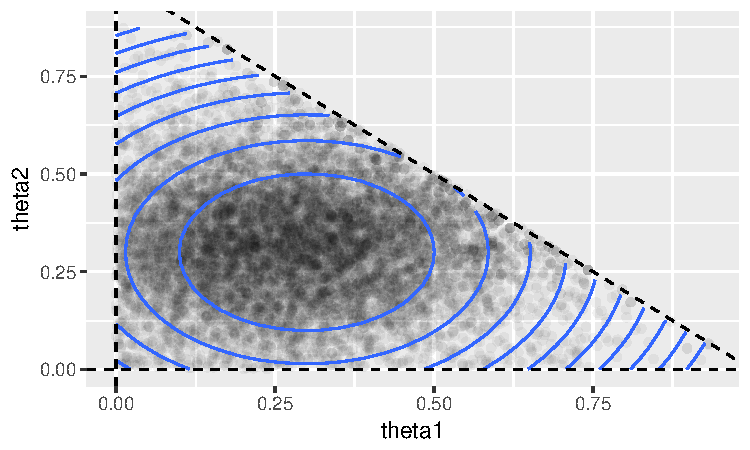
\includegraphics[width=1\textwidth]{linear_inequal_1}
\caption{Constrained $\No([0.3,0.3],1/{10})$}
\end{subfigure}
\begin{subfigure}[b]{0.45\textwidth}
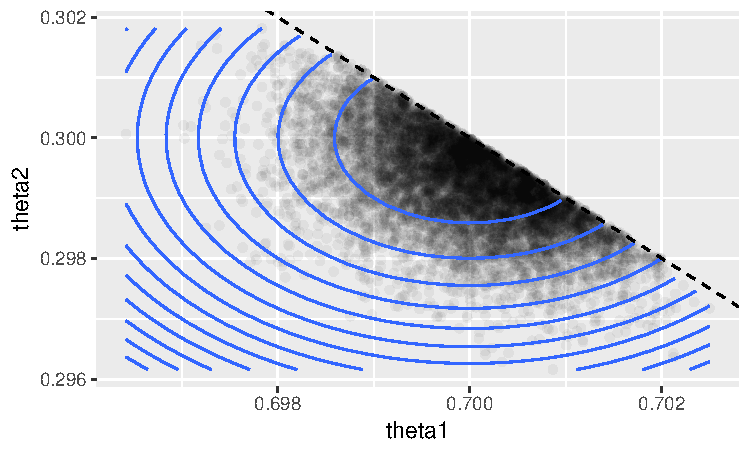
\includegraphics[width=1\textwidth]{linear_inequal_2}
\caption{Constrained $\No([0.7,0.3],1/{10^4})$}
\end{subfigure}
\caption{Posterior sample of bivariate normal distribution subject to linear inequality constraints $\theta\in(0,1)^2,\theta_1+\theta_2<1$, using HMC with  constraint relaxation. Posterior is spread out around the center (panel (a)) or concentrated on the boundary (panel (b)) of the region.}
\label{linear_inequality}
\end{figure}

To illustrate equality constraint relxation, we generate a simple von Mises--Fisher distribution $\pi_{\mc D}(\theta) \propto \exp(F'\theta)$ on a unit cirlce $\{(\theta_1,\theta_2):\theta_1^2+\theta_2^2=1\}$. We use $F=(1,1)$ to induce a relatively spread-out  $\theta$ on the manifold and $\exp(-\frac{|\theta'\theta -1|}{\lambda})$ for constraint relxation. As $\eta_{\mc D}=0$ on the circle, limiting the stability bound of leap--frog, some support expansion through moderate $\lambda$ is needed. This involves a trade-off between accuracy and speed. We test $\lambda = 10^{-3}$, $10^{-4}$ and $10^{-5}$ in three experiments. 
Table~\ref{table_circle} shows the computing time per $1,000$ effective sample size, the effective `violation' $|v(\theta)|=|\theta_1+\theta_2-1|$ and the 1-Wasserstein distance $W_1$ from its relxation approximate to the exact posterior, obtained using `movMF' package. As $W_1$ is numerically computed, we calculate the average distance comparing two independent samples from the same exact distribution, using it as reference. The distance $W_1$ based on $\lambda= 10^{-5}$ approximation is indistinguishable from this low numerical error, while the other has slightly larger error using shorter computing time.

%To visualize effects of stability bound, we restrict the maximum leap-frog steps $L$ to be $100$ and show how much space each setting can explore within one HMC iteration. Figure~\ref{unit_circle} plots its path of $L=100$ leap-frog steps.
% \begin{figure}[H]
% \centering
% \begin{subfigure}[b]{0.8\textwidth}
% 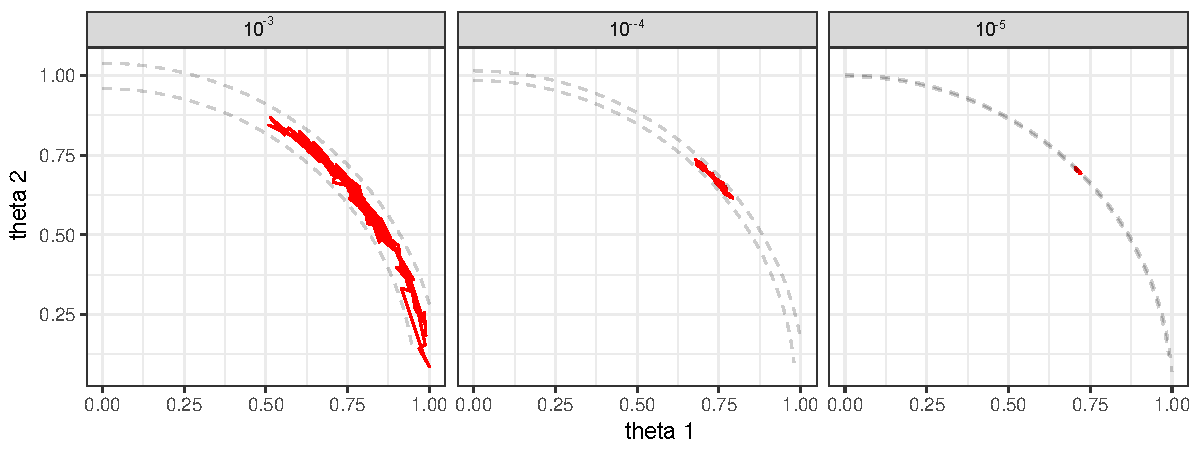
\includegraphics[width=1\textwidth]{unit_circle_100steps}
%       \end{subfigure}
%      \caption{Path of 100 itegrator steps in one HMC iteraton, sampling on a unit circle via extrinc prior with $\mc K(\theta)=\exp(-\frac{|\theta'\theta -1|}{\lambda})$, with $\lambda=10^{-4}$, $=10^{-5}$ and $=10^{-6}$. Larger relaxation in the narrowest direction of support (orthogonal vector to the circle) result in more efficient space exploration.}
%    \label{unit_circle}
%    \end{figure}


   \begin{table}[H]
   \begin{center}
   \footnotesize
   \begin{tabular}{ c| c | c| c | c}
   \hline			
   $\lambda$  &  $10^{-3}$ & $10^{-4}$ & $10^{-5}$ & Exact  \\
   \hline
   \hline
   $W_1$ & 0.050 & 0.034  & 0.014   & 0.015 \\

   &  (0.019, 0.095) &(0.027, 0.037) &  (0.013,0.025)  & (0.0014,0.025)\\

   \hline
   $|v(\theta)| \mid y$ 
   & $9\times 10^{-4} $ 
   & $9\times 10^{-5} $ 
   & $9\times 10^{-6} $ \\
   & $(2.6 \cdot 10^{-5}, 3.3\cdot 10^{-3})$& $(2.0 \cdot 10^{-6}, 3.4\cdot 10^{-4})$& $(2.7 \cdot 10^{-7}, 3.5\cdot 10^{-5})$& 0\\
   \hline
   Avg. Time (sec/1000 eff. sample) & 4.6 & 15.3 & 40.5 &    \\
   \hline  
   \end{tabular}
   \end{center}
   \caption{Average approximation error (with 95\% credible interval, out of $10$ repeated experiments) of sampling using constraint relaxtion for 
   a von--Mises Fisher distribution on a unit circle. At $10^{-5}$, the approximation is close to the limit of numeric error of numeric $W_1$.   The needed computing time increases about $3$ times when accuracy increases $10$ times. \label{table_circle}}
   \end{table}

   \section{Simulations and Applications}

   \subsection{Benchmark against Existing Approaches}

   We first benchmark the computing performance of the proposed
   constraint relaxation approach with existing state-of-art competitors.
   Bingham--von Mises--Fisher distribution is routinely used for such
   purpose, with $\pi_{\mc D}(\theta)\propto \exp(B'\theta+
   \theta'A\theta)$. We compare the performance with the Gibbs sampler
   \citep{hoff2009simulation} and  the geodesic HMC
   \citep{byrne2013geodesic}. The distribution is set to
   $A=\diag(-1000,-600,-200,200,600,1000)$ and $B=(100,0,0,0,0,0)$.

   We show that 


   \subsection{Application: Sparse Bases Learning}


   We now consider a real data application in brain network analysis. The brain connectivity structures are obtained in the data set KKI-42 (Landman et al. 2011), which consists of $21$ healthy subjects without any history of neurological disease. Each subject has two brain network observations from scan--rescan, yielding a total of n = 42. Each observation is a $V\times V$ symmetric network $A_i$, recorded as adjacency matrix $A_i$ for $i=1,\ldots,n$. For the $i$th matrix $A_i$, $A_{i,k,l} \in \{0,1\}$ is the element on the $k$th row and $l$th column of $A_i$, with $A_{i,k,l}=1$ indicating there is an connection betwen $k$th and $l$th region, $A_{i,k,l}=0$ if there is no connection. The regions are constructed via the Desikan et al. (2006) atlas, for a total of V = 68 nodes.

   The ambient dimension of observation is $V(V-1)/2=2,278$, which is significantly larger than sample size $n=40$. They potentially contain observational error in recording connectivity, and the  diagonal in each $A_{i}$ is missing due to the lack of self-connectivity. These facts motivate a Bayesian low-rank approach. We consider a symmetric tensor decomposition model:

   \begin{equation*}
   \begin{aligned}
   & A_{i,k,l} \sim \text{Bern}( \frac{1}{1+ \exp(-\psi_{i,k,l}- Z_{k,l})})\\
   & \psi_{i,k,l} = \sum_{r_1=1}^{d_1}\sum_{r_2=1}^{d_2} D_{r_1,r_2} W_{i,r_2} U_{k,r_1} U_{l,r_1}  \\
   \end{aligned}
   \end{equation*}
   for $k>l$, $k=2,\ldots, V$, $i=1,\ldots,n$; $U$ is $V\times d_1$ matrix, $W$ is $n\times d_2$ matrix; $D$ is a $d_1\times d_2$ array. The  $V\times V$ matrix $Z$ is almost unstructural except symmetric $Z_{k,l}=Z_{l,k}$, which is commonly used to induce low-rank in the decomposition \citep{durante2016nonparametric}.


   This model is a special Tucker decomposition with a sparse core tensor, whose diagonal plane is equal to $D$ and $0$ for other elements. The Tucker decomposition is more flexible than another routinely used decomposition, namely parallel factor analysis (PARAFAC). The PARAFAC assumes all ranks are equal and the core tensor $D$ only has non-zero value when all its sub-indices are equal. In this case, PARAFAC would assume $d_1=d_2$. The additional flexibility in the Tucker is appealing, as one could utilize the varying rank over different sub-direction (mode) of the tensor. On the other hand, a completely unconstrained Tucker decomposition is not identifiable in the matrices and core tensor, due scaling. For example, one can multiply a $d_1\times d_1$ non-zero diagonal matrix $R$, to $U$ and obtain $U^*=UR$ obtain $D^{*}_{.,r_2,.}=R^{-1}D_{.,r_2,.}R^{-1}$ for $r_2=1,\ldots,d_2$. This leaves the likelihood unchanged, creating identifiability issue. 

   Therefore, we consider applying some constraint on the Tucker decomposition. Motivated by high-order singular value decomposition, we impose orthonormality constraints $U'U=I_{d_1}$ and $W'W=I_{d_2}$. \cite{hoff2016equivariant} previously obtained conjugated posterior for Tucker decomposition under orthonormality constraint, however, the symmetry in undirectedness of networks breaks the conjugacy.

   We assign normal prior for $U_{k,r_2}\sim \No(0,\phi_{1})$, $W_{i,r_1}\sim \No(0,\phi_2)$, $Z_{k,l}\sim \No(0,\phi_3)$, $D_{r_1,r_2}\sim No(0, \phi_{4,r_1,r_2})$ for all $i,k,l,r_1,r_2$, and inverse-Gamma prior $\phi_1,\phi_2,\phi_3\stackrel{indep}{\sim} \text{IG}(2,1)$, $\phi_{4,r_1,r_2}= \tau_{r_1}\tau_{r_2}$, with $\tau_{r_1},\tau_{r_2}\stackrel{indep}{\sim} \text{IG}(2,1)$ for all $r_1,r_2$. We

%we assign multiplicative inverse gamma distribution \citep{bhattacharya2011sparse} $\phi_{4,r_1,r_2}= \prod_{m_1=1}^{r_1} \nu_{1,m_1} \prod_{m_2=1}^{r_2}  \nu_{2,m_2}$ with $\nu_{1,1},\nu_{2,1} \stackrel{indep}{\sim} \text{IG}(a_1,1)$ and $\nu_{1,m},\nu_{2,m}\stackrel{indep}{\sim} \text{IG}(a_2,1)$ for $m\ge 2$. This induces increasing concentration toward zero as $r_1,r_2$ increase, allowing adaptive choosing of latent dimensions. We set $a_1=a_2=5$ in this application.

To allow estimation for model with orthonormality constraint, we use extrinsic prior with $\mc K(\theta) = \exp( - \frac{(U'U-I_{d_1})^2 + (W'W-I_{d_2})^2  }{\lambda})$ and set $\lambda=10^{-3}$. To compare, we also test with the same model configuration without the orthonormality constraint. We run both models for $10,000$ steps and discard the first $5,000$ steps. Figure~\ref{tucker} plots the traceplot and autocorrelation for matrix $U$. Unconstrained base model has severe convergence issue due to the non-identifiability, while constrained model converges and show low autocorrelation for all the parameters.

\begin{figure}[H]
\begin{subfigure}[b]{1\textwidth}
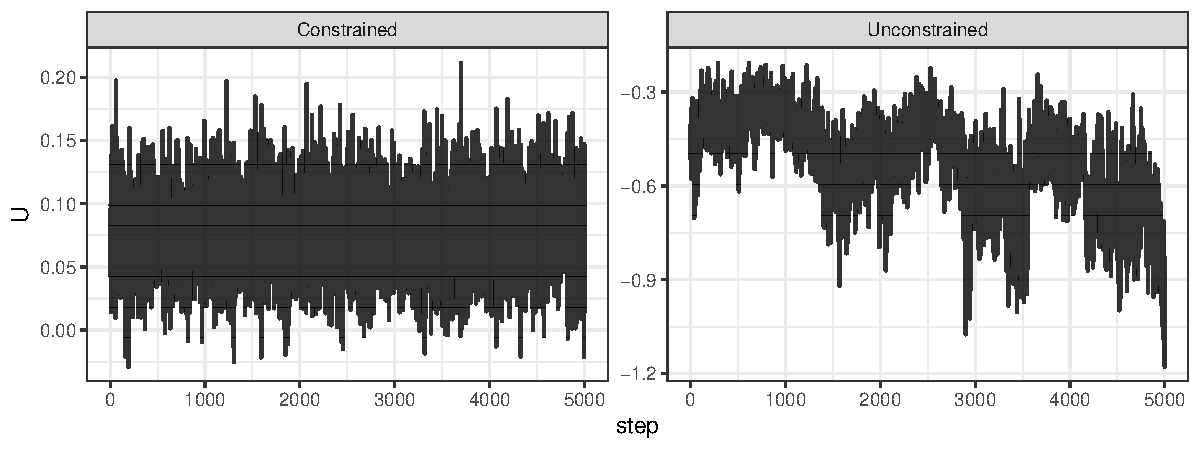
\includegraphics[width=1\textwidth]{tucker_traceplot.pdf}
\caption{Traceplot of $U_{1,1}$.}
\end{subfigure}
\begin{subfigure}[b]{1\textwidth}
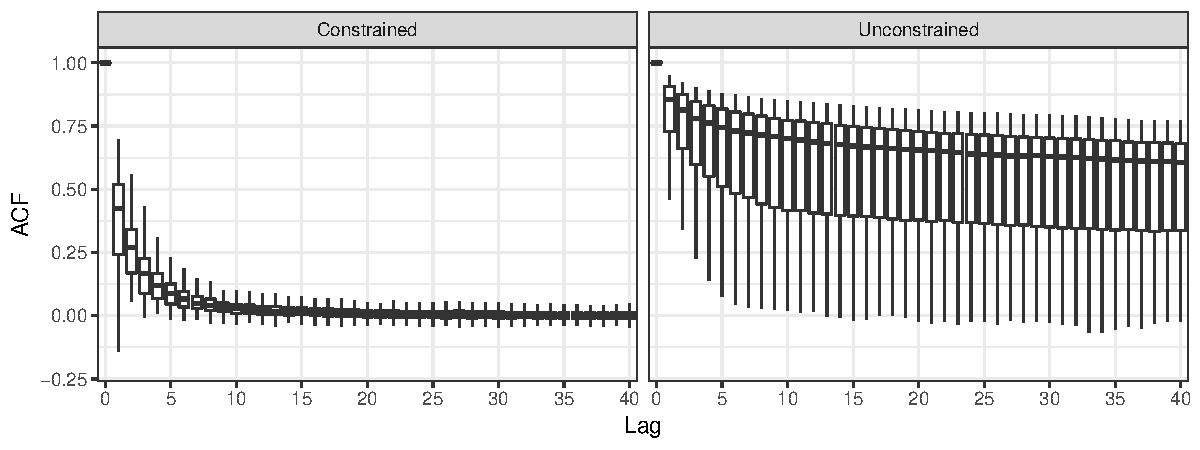
\includegraphics[width=1\textwidth]{tucker_acf.pdf}
\caption{ACF of all elements in $U$}
\end{subfigure}
\caption{Orthonormality constraint in the tensor decomposition modelallows convergence and rapid mixing on the factor matrix (left column); whereas unconstrained model does not converge due to free scaling. Traceplot for one parameter in factor matrix $U$ and boxplot for autocorrelations of all parameters are shown.}
\label{tucker}
\end{figure}

\section{Discussion}

The estimation difficulty associated with parameter constraint often hinders the development of new models. Often one needed to carefully avoid models without conjugate posteriors, or skillfully re-parameterize the model for a more tractable algorithm. The extrinsic approach we introduced significantly reduces the burden. Through space expansion, it allows conventional toolbox such as HMC to be easily adopted to sample posterior without closed-forms. This allows researchers to impose constraints more freely in modeling and simplifies the way to incorporate constraint information about the functional of parameters.

We show the approximation error of the extrinsic approach can controlled via tuning parameter, with some trade-off between computing time and accuracy. A potentially more efficient strategy would be obtaining a rough approximate first in $\mc R$, then projecting into $\mc D$. \cite{lin2016extrinsic} developed algorithms similar to this idea and obtained consistency result for point estimation. A useful task would be to find an optimal projection also quantifying the uncertainty associated with finite sample. Lastly, the normalization of parameters over constrained space can sometime yield intractable integral, known as `doubly stochastic' problem. We expect that the proposed extrinsic prior can be adapted and used together with the various existing solutions \citep{rao2016data,stoehr2017noisy}.



\bibliography{reference}
\bibliographystyle{chicago}

\section{Appendix}

Remark 1 proof:
\begin{proof}[Proof]
Let $g:\mathbb{R}^p\rightarrow \mathbb{R}$ be a 1-Lipschitz continuous function, i.e. $\|g(x)-g(y)\|\le \|x-y\|$, denoted by $\|g\|_L\le 1$. 
By Kantorovich-Rubinstein duality, the 1-Wasserstein distance based on Euclidean metric equals to: 

\begin{equation}
W_1(\Pi,\tilde\Pi)=\underset{g:\|g\|_L\le 1}\sup \int g(x) \Pi(dx) -  \int g(y) \tilde\Pi(dy) 
\end{equation}

Taking $g(\theta)=\exp(-\lambda^{-1}v(\theta))$ yields
\begin{equation}
\begin{aligned}
m_\lambda
& = \int_\mathbb{R}  \left[ \int_{v^{-1}(x)} \frac{ \exp(- \lambda^{-1} v(\theta) ) \pi_{\mc R}(\theta)}{ J v(\theta) } \mathcal{H}^{p-d}(d \theta) \right] \mathbbm{1}_{x \ge 0}  d x \\
& = \int_\mathbb{R}  m(x)\exp(- \lambda^{-1} x ) \mathbbm{1}_{x \ge 0}  d x .
\end{aligned}
\end{equation}

Taking $g(\theta)={\mathbbm{1}_{v(\theta)=0}}$ yields 
\begin{equation}
m_0
= \int_\mathbb{R} \left[ \int_{v^{-1}(y)} \frac{ \pi_{\mc R}(\theta) }{ J v(\theta) } \mathcal{H}^{p-d}(d \theta) \right]\mathbbm{1}_{y=0} dy   =  \int_{v^{-1}(0)} \frac{ \pi_{\mc R}(\theta) }{ J v(\theta) } \mathcal{H}^{p-d}(d \theta) =m(0)
\end{equation}

Clearly $m_\lambda \ge m_0$.

1. Asymptotic result:

We have

\begin{equation}		
\label{wass0}
\begin{aligned}
&\underset{g:\|g\|_L\le 1}\sup\int g(\theta)  \left[ \frac{ \exp(- \lambda^{-1} v(\theta)) } {  m_\lambda}  - 
\frac{ \mathbbm{1}_{v(\theta)=0} } {  m_0} 
\right]  \frac{\pi_{\mc R}(\theta)}{Jv(\theta)} \mc H^{p-d}(d \theta) \\
&= \underset{g:\|g\|_L\le 1}\sup\int_\mathbb{R}  \mathbb{E}(g(\theta) \mid x)  \left[ \frac{ \exp(- \lambda^{-1} x) \mathbbm{1}_{x \ge 0}} {  m_\lambda}  - 
\frac{ \mathbbm{1}_{x=0} } {  m_0} 
\right] d x \\
&=	\underset{g:\|g\|_L\le 1}\sup\int_\mathbb{R}  \mathbb{E}(g(\theta) \mid x)  \left[ \frac{  1} {  m_\lambda}  - 
\frac{ 1 } {  m_0} 
\right]\mathbbm{1}_{x=0} d x  + \underset{g:\|g\|_L\le 1}\sup\int_\mathbb{R}  \mathbb{E}(g(\theta) \mid x)\frac{ \exp(- \lambda^{-1} x)} {  m_\lambda}  
\mathbbm{1}_{x > 0} d x \\
& \le \underset{g:\|g\|_L\le 1}\sup \|\mathbb{E}(g(\theta) \mid 0)\| \left[ \frac{ 1 } {  m_0} -\frac{  1} {  m_\lambda}   
\right] + \frac{1} {  m_0} \underset{g:\|g\|_L\le 1}\sup \int_\mathbb{R}  \|\mathbb{E}(g(\theta) \mid x)\| { \exp(- \lambda^{-1} x)}
\mathbbm{1}_{x > 0} d x \\	
\end{aligned}
\end{equation}


Note $m_\lambda\le \int_\mathbb{R} m(x) \mathbbm{1}_{x \ge 0}  dx =\int_\mathbb{R} \pi_{\mc R}(\theta) =1$. By dominated convergence theorem, 

\begin{equation}
\lim_{\lambda\rightarrow 0}m_\lambda= \int_\mathbb{R}  m(x) \lim_{\lambda\rightarrow 0}\exp(- \lambda^{-1} x ) \mathbbm{1}_{x \ge 0}  d x = m_0.
\end{equation}


Since 
$ \underset{g:\|g\|_L\le 1}\sup \int_\mathbb{R}  \|\mathbb{E}(g(\theta) \mid x)\| { \exp(- \lambda^{-1} x)} dx \le \int_\mathbb{R} \underset{g:\|g\|_L\le 1}\sup \|\mathbb{E}(g(\theta) \mid x)\| { \exp(- \lambda^{-1} x)} dx$,
letting $q_\lambda=	  \underset{g:\|g\|_L\le 1}\sup \|\mathbb{E}(g(\theta) \mid x)\| { \exp(- \lambda^{-1} x)}
\mathbbm{1}_{x > 0}  $, we have $0\le q_1-q_{\lambda_1}\le q_1-q_{\lambda_2}$ for $1\ge\lambda_1\ge \lambda_2$, by monotone convergence theorem, $\lim_{\lambda\rightarrow 0}\int [ q_1(x)-q_\lambda(x)]dx = \int [q_1(x)- q_0(x) ]dx$ hence $\lim_{\lambda\rightarrow 0}\int q_\lambda(x)dx =0$. Combining the results yields 



\begin{equation}
\underset{\lambda \rightarrow 0}\lim W_1(\Pi,\tilde\Pi)=0.	  \end{equation}

2. Non-asympotic result:


\begin{equation}
\label{wass1}
\begin{aligned}
\frac{1}{m_0}-\frac{1}{m_\lambda} & \le  \frac{   \int_\mathbb{R}  m(x) \exp(- \lambda^{-1} x ) \mathbbm{1}_{x > 0}  d x } {  m_0^2}  \\
&= \frac{1}{ m_0^2} \left[ \int_0^{t}  m(x) \exp(- \lambda^{-1} x ) dx + \int_t^{\infty}  m(x) \exp(- \lambda^{-1} x ) dx \right] \\
&\le \frac{1}{ m_0^2} \left[  \underset{t^*\in (0,t)}\sup m(t^{*})\int_0^{t} \exp(- \lambda^{-1} x ) dx + \exp(- \lambda^{-1} t )\int_t^{\infty}  m(x) dx  \right] \\
&\le \frac{1}{ m_0^2} \left[\lambda \underset{t^*\in (0,t)}\sup  m(t^{*})  + \exp(- \lambda^{-1} t ) \right] 
\end{aligned}
\end{equation}

\begin{equation}
\label{wass2}
\begin{aligned}
& \underset{g:\|g\|_L\le 1}\sup\int_\mathbb{R}  \|\mathbb{E}(g(\theta) \mid x)\| { \exp(- \lambda^{-1} x)}	\mathbbm{1}_{x > 0} d x \\
&\le \underset{g:\|g\|_L\le 1}\sup\underset{t^*\in (0,t)}\sup \|\mathbb{E}(g(\theta) \mid t^*)\|	
\int_0^{t} \exp(- \lambda^{-1} x ) dx + \exp(- \lambda^{-1} t ) \underset{g:\|g\|_L\le 1}\sup \int_t^{\infty}   \|\mathbb{E}( g(\theta )\mid x)\| dx \\
&\le \underset{g:\|g\|_L\le 1}\sup\underset{t^*\in (0,t)}\sup \|\mathbb{E}(g(\theta) \mid t^*)\|	\lambda + \exp(- \lambda^{-1} t ) \underset{g:\|g\|_L\le 1} \sup \mathbb{E}(\| g(\theta )\|) \\
\end{aligned}
\end{equation}

Combining \eqref{wass0}\eqref{wass1}\eqref{wass2}, $k_1=\underset{g:\|g\|_L\le 1}\sup\underset{t^*\in [0,t)}\sup \|\mathbb{E}(g(\theta) \mid t^*)\|$, $k_2=\underset{g:\|g\|_L\le 1} \sup \mathbb{E}(\| g(\theta )\|)$, $k_3= \underset{t^*\in (0,t)}\sup  m(t^{*})$


\begin{equation}
\begin{aligned}
& \underset{g:\|g\|_L\le 1}\sup \int g(x) \Pi(dx) -  \int g(x) \tilde\Pi(dx) \\
	%&\le  \frac{k_1}{ m_0^2} \left[\lambda k_3  + \exp(- \lambda^{-1} t ) \right] 
	%+ \frac{1} {  m_0} [ k_1	\lambda + \exp(- \lambda^{-1} t )k_2 ]\\	
	& \le \lambda (\frac{k_1 k_3}{m_0^2} + \frac{k_1}{m_0}) + \exp(- \lambda^{-1} t )(\frac{k_1}{m_0^2} + \frac{k_2}{m_0})
	\end{aligned}
	\end{equation}


	\end{proof}
	\end{document}
